\setcounter{section}{0}
\section{Hình thành kiến thức mới}

\subsection{Mở đầu}
Chuyên đề "Vật lí với giáo dục và bảo vệ môi trường" đề cập đến một trong những vấn đề thời sự của thực tiễn: sự tàn phá môi trường đang ảnh hưởng nghiêm trọng đến sự phát triển bền vững của từng quốc gia, đặc biệt là ở nước ta. Các nhiệm vụ tìm hiểu trong chuyên đề sẽ giúp bạn có nhận thức đúng đắn và hành động phù hợp để bảo vệ môi trường, thích ứng với biến đổi khí hậu, đáp ứng nhu cầu phát triển bền vững.
\subsection{Hình thành kiến thức mới}

\subsubsection{Môi trường - Ô nhiễm môi trường}
\begin{center}
	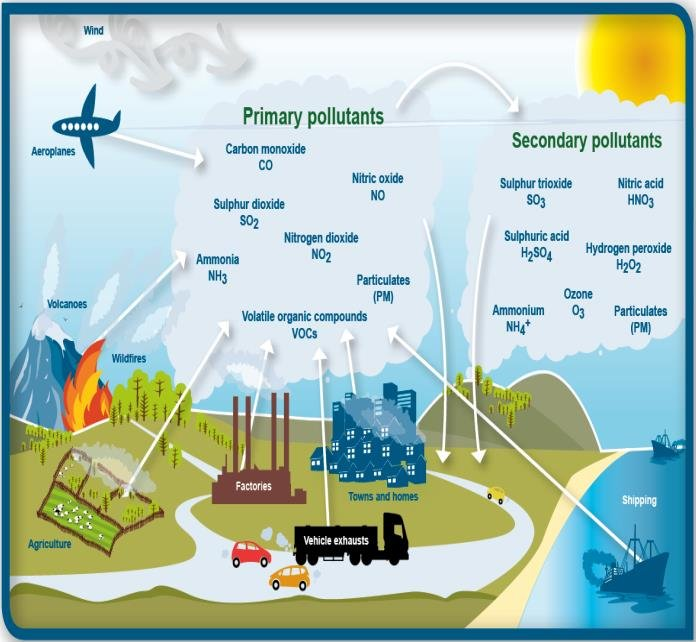
\includegraphics[width=0.6\linewidth]{../figs/G10-036-2}
\end{center}
Môi trường bao gồm các yếu tố tự nhiên và nhân tạo bao quanh con người, có mối quan hệ mật thiết với nhau, ảnh hưởng lớn đến đời sống, sản xuất, sự tồn tại cũng như phát triển của con người và thiên nhiên.
\begin{itemize}
	\item Môi trường tự nhiên bao gồm các thành phần tự nhiên như địa hình, địa chất, đất trồng, khí hậu, sinh vật, nước, $\ldots$.
	\item Môi trường xã hội chính là tổng thể các mối quan hệ xã hội giữa con người với con người thông qua hệ thống luật pháp, thể chế, quy định, cam kết, $\ldots$.
	\item Môi trường nhân tạo chính là các đối tượng lao động do con người sản xuất ra và chịu sự chi phối của con người.
\end{itemize}

Ô nhiễm môi trường là việc thâm nhập các chất làm hại cho sức khỏe của sinh vật vào môi trường. Các chất này có thể từ thiên nhiên (như khói bụi từ núi lửa phun ra) hoặc được sinh ra bởi các hoạt động của con người. Có ba dạng ô nhiễm chính: ô nhiễm đất, ô nhiễm nước và ô nhiễm không khí.

Ngoài ra, ô nhiễm ánh sáng và ô nhiễm tiếng ồn cũng gây ra những ảnh hưởng xấu đến sức khỏe, sinh hoạt và chu kì sinh học của con người cũng như các loài động, thực vật.
\subsubsection{Bảo vệ môi trường}
Để giải quyết vấn đề ô nhiễm môi trường, các quốc gia và các tổ chức quốc tế đã xây dựng chiến lược bảo vệ môi trường. Các kế hoạch, chương trình, biện pháp hành động cụ thể như: quản lí chất thải rắn; giảm các loại rác nhựa; quản lí và cải thiện môi trường liên quan đến nước thải, hóa chất trong nông nghiệp; nuôi trồng thủy sản và công nghiệp, chất thải công nghiệp; xử lí nước thải; quản lí rừng, tài nguyên khoáng sản; tăng cường trồng rừng để gia tăng độ che phủ rừng; tuyên truyền bảo vệ môi trường và sẵn sáng thích ứng với thiên tai.

\subsubsection{Sử dụng nhiên liệu hóa thạch}
Nhiên liệu hóa thạch như than đá, dầu mỏ, khí thiên nhiên, $\ldots$ được hình thành nhờ sự phân hủy xác động vât, thực vật và quá trình biến đổi của địa chất trong hàng triệu năm.

Than đá là nguồn năng lượng chủ yếu trong các ngành nhiệt điện, xi măng, luyện kim và phân bón. Than đá cháy trong không khí tỏa ra nhiều nhiệt, nhưng thải ra nhiều loại khí độc như SO$_2$, CO, NO$_2$, $\ldots$ và bụi mịn gây hại cho phổi, tim và hệ thần kinh của con người.
\subsubsection{Sử dụng năng lượng tái tạo}
\begin{center}
	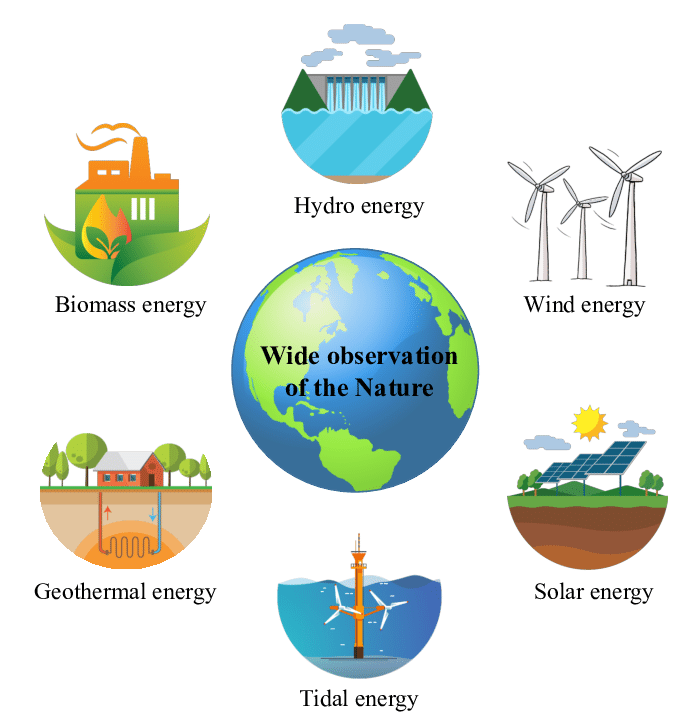
\includegraphics[width=0.5\linewidth]{../figs/G10-036-1.png}
\end{center}
Năng lượng tái tạo là dạng năng lượng được cung cấp bởi những nguồn nguyên liệu có sẵn trong tự nhiên và không bao giờ cạn kiệt hoặc có thời gian sử dụng rất lớn như năng lượng Mặt Trời, gió, nước, thủy triều, địa nhiệt, sinh khối, $\ldots$.

Năng lượng tái tạo có vai trò quan trọng trong sự phát triển kinh tế, xã hội và bảo vệ môi trường để đảm bảo phát triển bề vững. Cụ thể là:
\begin{itemize}
	\item Năng lượng tái tạo có trữ lượng vô hạn, có tiềm năng thay thế các nguồn năng lượng hữu hạn như năng lượng hóa thạch, góp phần tránh được các hậu quả có hại đến môi trường.
	\item Việc phát triển năng lượng tái tạo được xem là bước đi tiên phong cho việc giảm khí thải gây ra hiệu ứng nhà kính.
	\item Việc sử dụng năng lượng tái tạo góp phần tăng cường nguồn cung trong nước, giảm thiểu sự phụ thuộc vào nguồn năng lượng nhập khẩu nước ngoài, đảm bảo an ninh năng lượng quốc gia.
\end{itemize}

Một số công nghệ cơ bản để thu được năng lượng tái tạo:
\begin{itemize}
	\item Điện Mặt Trời: sử dụng pin Mặt Trời biến đổi năng lượng ánh sáng Mặt Trời thành điện năng. Quá trình chuyển hóa năng lượng này xảy ra theo các giai đoạn sau: ánh sáng Mặt Trời chiếu tới làm xuất hiện các hạt mang điện trong tấm bán dẫn, dưới tác dụng của một hiệu điện thế, các hạt mang điện này chuyển động có hướng để tạo thành dòng điện.
	\item Nhiệt Mặt Trời: Quang năng từ bức xạ Mặt Trời được chuyển hóa thành nhiệt năng sử dụng trong một số thiết bị như: bếp, máy nước nóng sử dụng năng lượng Mặt Trời.
	\item Năng lượng gió: Năng lượng gió có thể chuyển thành cơ năng trong cối xay gió hoặc sử dụng gián tiếp thông qua các thiết bị chuyển đổi như tuabin gió để chuyển thành năng lượng điện.
	\item Năng lượng sinh khối: Đê chuyển năng lượng sinh khối thành điện năng, ta có thể sử dụng một số phương pháp như: đốt trực tiếp và sử dụng lò hơi; đôt liên kết; nhiệt phân.
	\item Năng lượng nước: Thế năng trọng trường của nước được tích lũy tại các đập thủy điện ở trên cao. Sau khi nước được xả ra và chảy xuống dưới, động năng của nó làm quay tuabin và phát ra điện.
	\item Năng lượng đại dương: Bao gồm năng lượng thủy triều, năng lượng sóng, năng lượng nhiệt đại dương.
	\item Năng lượng địa nhiệt: từ các nguồn đá nóng, nước nóng ngầm dưới đất như núi lửa, suối nước nóng, hồ nước nóng.
\end{itemize}
\subsubsection{Sử dụng năng lượng ở Việt Nam hiện nay}
Trong những năm qua, Việt Nam là nền kinh tế năng động, phát triển khá nhanh. Ngành năng lượng đóng vai trò then chốt trong việc thúc đẩy phát triển kinh tế - xã hội.

Hiện nay, năng lượng thủy điện đã gần như khai thác hết, trữ lượng than đá cũng đang cạn dần. Việc sử dụng nhiều năng lượng hóa thạch cũng gây ô nhiễm môi trường.

Việc sử dụng năng lượng không hiệu quả gây nhiều hiện tượng khí hậu cực đoan như nắng nóng khắc nghiệt, cháy rừng, lũ lụt, bão lũ đã ảnh hưởng đến hàng triệu người, đồng thời gây ra những hiểm họa đối với sức khỏe, an ninh và phát triển kinh tế. Việt Nam là nước chịu thiệt hại nặng nề nhất của biến đổi khí hậu. So sánh với một số nước đang phát triển chịu tác động của biến đổi khí hậu thì Việt Nam là quốc gia chịu thiệt hại tính trên GDP cao nhất.

Trong tương lai, Việt Nam cần khai thác hợp lí, hiệu quả và sử dụng nguồn năng lượng hiện có, mở rộng khai thác các nguồn năng lượng tái tạo, thân thiện với môi trường.


\subsection{Mở rộng}
\subsubsection{Vai trò của cá nhân và cộng đồng trong bảo vệ môi trường}
Việc bảo vệ môi trường không chỉ là nhiệm vụ quốc gia mà bản thân môi cá nhân, cộng đồng có cách bảo vệ môi trường thiết thực nhất, có thể kể đến như:
\begin{itemize}
	\item Phân loại rác thải.
	\item Hạn chế sử dụng thuốc bảo vệ thực vật, các loại hóa chất, chất thải gây ô nhiễm môi trường, $\ldots$
	\item Sử dụng tiết kiệm điện, hạn chế các phương tiện giao thông cá nhân, tăng cường sử dụng năng lượng sạch.
	\item Trồng nhiều cây xanh, hạn chế chặt phá rừng.
	\item Tuyên truyền, vận động gia đình, cộng đồng tham gia bảo vệ môi trường.
\end{itemize}

\subsubsection{Sử dụng năng lượng hiệu quả trong đời sống và sản xuất}
Sử dụng năng lượng hiệu quả là mục tiêu của những nỗ lực nhằm giảm năng lượng cần thiết cung cấp cho sản xuất và dịch vụ.

Việc sử dụng điện sinh hoạt quá mức như máy điều hòa, tủ lạnh tiêu tốn nhiều năng lượng. Các máy làm lạnh là thiết bị dùng để chuyển nhiệt lượng từ nơi lạnh sang nơi nóng bằng cách sử dụng điện năng để nén và dãn nở khí làm nhiệt độ của nó tăng lên và truyền ra môi trường.

Điều hòa nhiệt độ là thiết bị sử dụng điện năng giúp hạ nhiệt độ hoặc tăng nhiệt độ trong phòng. Việt thiết kế công trình, lắp đặt và sử dụng điều hòa hợp lí sẽ giúp tiết kiệm điện năng.

Tủ lạnh là một thiết bị làm mát, gồm ngăn cách nhiệt và hệ thống để truyền nhiệt từ nó ra môi trường bên ngoài. Tủ lạnh có thể duy trì nhiệt độ trong ngăn cách nhiệt ở nhiệt độ lạnh nhất định.

Để sử dụng tủ lạnh tiết kiệm điện cần bố trí tủ ở nơi thoáng mát và sử dụng hợp lí.

Bình nước nóng là một thiết bị điện gia dụng cung cấp nguồn nước nóng dựa vào việc chuyển điện năng thành nhiệt năng khi cho dòng điện chạy qua dây dẫn. Lựa chọn và sử dụng bình nước nóng không hợp lí sẽ tiêu hao nhiều điện năng.

Xe máy, ô tô, máy phát điện, $\ldots$ sử dụng nhiên liệu đốt trong xi lanh của động cơ làm hệ thống động cơ nóng lên. Hệ thống làm mát của động cơ rất quan trọng. Nếu hệ thống làm mát bám bụi bẩn, không được bổ sung nước làm mát đầy đủ sẽ ảnh hưởng đến quá trình thải nhiệt ra môi trường, khiến nhiệt độ buồng máy tăng cao. Hiệu suất động cơ sẽ thấp và tốn nhiên liệu. Vì vậy, nên vệ sinh sạch sẽ, bổ sung nước làm mát đầy đủ cho một số động cơ.
\subsubsection{Thiết kế tuabin gió mini}

\begin{minipage}{0.6\textwidth}
	Yêu cầu:
	\begin{itemize}
		\item Thiết bị tạo ra được hiệu điện thế và dòng điện một chiều.
		\item Thời gian chế tạo tối đa 20 phút, chỉ sử dụng những vật liệu được cung cấp: 01 động cơ điện một chiều, dây điện, ống nước, tấm bìa, đũa tre, kéo, keo nến, đồng hồ đo điện, thước kẻ, thước đo độ, bút chì, quạt điện nhỏ tạo nguồn gió.
		\item Nghiên cứu ảnh hưởng của cánh quạt (chiều dài, độ nghiêng, số lượng) tới điện áp ra của tuabin.
	\end{itemize}
	
	Cách thức tiến hành:
	\begin{itemize}
		\item Thiết kế khung đế và giá đỡ cho tuabin.
		\item Thiết kế cánh quạt.
		\item Lắp cánh quạt vào trục tuabin.
		\item Đấu nối dây điện vào tuabin để lấy điện ra.
	\end{itemize}
\end{minipage}
\begin{minipage}{0.4\textwidth}
	\begin{center}
		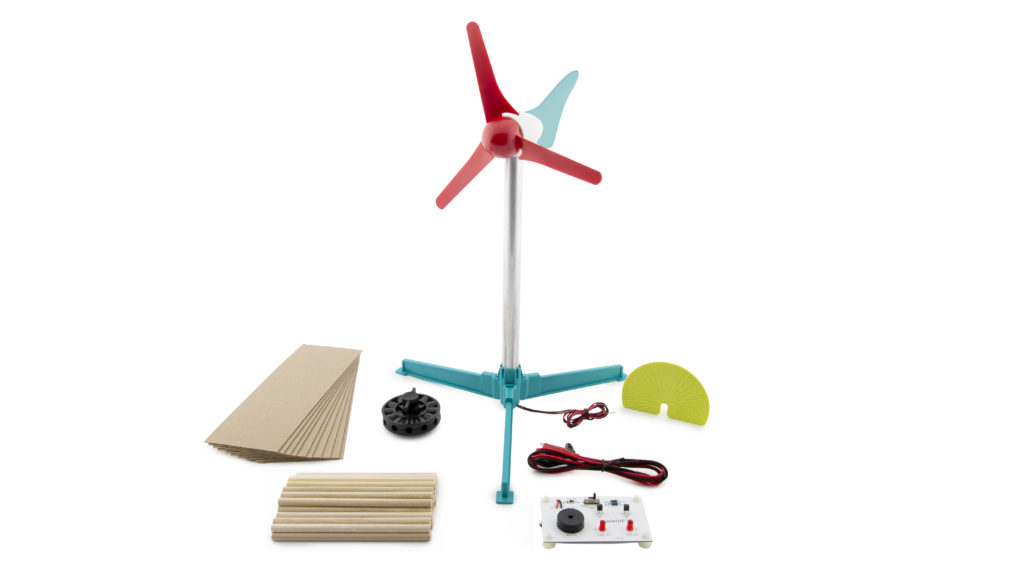
\includegraphics[width=\textwidth]{../figs/G10-036-3}
	\end{center}
\end{minipage}

\section{Mục tiêu bài học - Ví dụ minh họa}

\begin{dang}{Hiểu được tầm quan trọng của môi trường \\và ý nghĩa của việc bảo vệ môi trường}
	\viduii{2}{Môi trường có vai trò quan trọng như thế nào đối với đời sống con người?
	}
	{	\begin{center}
			\textbf{Hướng dẫn trả lời}
		\end{center}
		
		Môi trường sống tạo ra không gian sống, cung cấp nguồn tài nguyên thiên nhiên cũng như là như là nơi chứa đựng các chất thải do con người tạo ra trong hoạt động sinh hoạt và sản xuất. Môi trường sống trong lành thì sức khỏe con người mới được đảm bảo.
		
		
	}
	\viduii{2}{Môi trường sống của con người đang bị tác động tiêu cực như thế nào?
	}
	{	\begin{center}
			\textbf{Hướng dẫn trả lời}
		\end{center}
		
		Môi trường sống của con người đang bị hủy hoạt nghiêm trọng mà nguyên nhân cũng bắt nguồn từ con người như khói bụi từ các khu công nghiệp, phương tiện giao thông, khai thác cạn kiệt khoáng sản, $\ldots$ gây ra sự nóng lên toàn cầu và biến đổi khí hậu, gây ra hiện tượng băng tan, lũ lụt, hạn hán.
	}
\end{dang}
\begin{dang}{Nêu được cách sử dụng năng lượng hiệu quả trong đời sống và sản xuất}
	\viduii{2}{Tại sao cần đặt dàn nóng điều hòa và tủ lạnh ở nơi thoáng mát?
	}
	{	\begin{center}
			\textbf{Hướng dẫn trả lời}
		\end{center}
		
		Dàn nóng thuộc khối bên ngoài nên thường được lắp đặt ở ngoài trời, thường xuyên phải đối mặt với các yếu tố bất lợi của thời tiết.
		
		Theo tiêu chuẩn khuyến cáo của các nhà sản xuất, dàn nóng máy lạnh cần đặt ở vị trí đảm bảo các yếu tố cơ bản như: Vị trí cố định chắc chắn, tránh rung lắc. Phía trong dàn tản nhiệt cách tường tối thiểu $15 - 20 \text{ cm}$, phía ngoài quạt dàn nóng phải có không gian đủ rộng rãi thông thoáng. Không đặt ở vị trí có không khí nóng, không cho ánh nắng mặt trời chiếu thẳng vào. Khoảng cách giữa dàn nóng và dàn lạnh không quá xa nhau, vị trí cần thuận lợi cho công tác sửa chữa, bảo trì.
		
		Với đặc tính xả thải nhiệt vô cùng lớn, nên đặt dàn nóng ở nơi thoáng mát để tạo điều kiện thuận lợi cho sự giải nhiệt, từ đó tiết kiệm năng lượng và tăng tuổi thọ cho thiết bị.
	}
	\viduii{2}{Hãy nêu một số biện pháp tiết kiệm năng lượng khi sử dụng các thiết bị điện trong gia đình em.
	}
	{	\begin{center}
			\textbf{Hướng dẫn trả lời}
		\end{center}
		
		Học sinh có thể kể đến vài phương pháp tiết kiệm năng lượng đơn giản, thiết thực sau:
		\begin{enumerate}
			\item Tăng nhiệt độ của tủ lạnh, điều hòa;
			\item Chọn những sản phẩm có dán nhãn tiết kiệm năng lượng;
			\item Không lạm dụng máy sưởi, máy điều hòa;
			\item Thường xuyên làm sạch và bảo dưỡng thiết bị;
			\item Dùng ít nước hơn, tái sử dụng nước sinh hoạt;
			\item Ưu tiên đi bộ, đi xe đạp đến những nơi gần nhà; ưu tiên sử dụng phương tiện công cộng;
			\item Cách nhiệt cho căn nhà, hiện đại hóa hệ thống cửa sổ;
			\item Đề xuất các giải pháp tiết kiệm năng lượng ở cơ quan, trường học và cộng đồng.
		\end{enumerate}
	}
\end{dang}
\begin{dang}{Nêu được những hành động thiết thực ứng phó với\\ sự suy giảm tầng ozone và biến đổi khí hậu}
	\viduii{2}{Hãy tìm hiểu các tác động sinh học bởi sự tăng cường tia cực tím do suy giảm tầng ozone. Cần có những hành động thiết thực nào để hạn chế sự suy giảm tầng ozone?
	}
	{	\begin{center}
			\textbf{Hướng dẫn trả lời}
		\end{center}
		
		Sự suy giảm tầng ozone là hiện tượng giảm lượng ozone trong tầng bình lưu. Lớp ozone có tác dụng ngăn cản phần lớn các tia cực tím có hại không cho xuyên qua bầu khí quyển Trái Đất, sự suy giảm ozone đang được quan sát thấy và các dự đoán suy giảm trong tương lai đã trở thành một mối quan tâm toàn cầu.
		
		Dưới tác động của tia cực tím các nguyên tử Cl được giải phóng khỏi các hợp chất. Các nguyên tử Cl phá hủy các phân tử ozone, làm giảm lượng ozone ở tầng bình lưu và tạo ra lỗ thủng ozone, hậu quả là cường độ tia cực tím ở bề mặt Trái Đất tăng lên và có thể gây hại cho sinh vật và môi trường trên Trái Đất như: gây ung thư da, hình thành các khối u, các bệnh về mắt ở con người; làm hủy hoại vi sinh vật gây mất cân bằng sinh thái; làm giảm chất lượng không khí gây ô nhiễm môi trường.
		
		Các biện pháp thiết thực hạn chế sự suy giảm tầng ozone:
		\begin{enumerate}
			\item Nghị định thư MONTREAL giảm phát thải khí CFC.
			\item Hằng năm tổ chức trồng cây gây rừng.
			\item Có các biện pháp thiết thực để bảo vệ rừng.
			\item Hạn chế sử dụng năng lượng hạt nhân.
			\item Sử dụng các loại năng lượng sạch như gió, ánh sáng Mặt Trời, sóng biển.
			\item Xử lí ô nhiễm các khu công nghiệp, nhà máy, các đô thị.
			\item Giáo dục tư vấn, tuyên truyền để bảo vệ tầng ozone.
			\item Sử dụng các phương tiện công cộng.
		\end{enumerate}
		
	}
	\viduii{2}{Hãy tìm hiểu sự biến đổi khí hậu hiện nay và tác động tiêu cực đến Việt Nam. Cần có những hành động thiết thực nào để hạn chế sự biến đổi khí hậu?
	}
	{	\begin{center}
			\textbf{Hướng dẫn trả lời}
		\end{center}
		
		Một cách tổng quát, biến đổi khí hậu là sự thay đổi của hệ thống khí hậu ở bề mặt Trái Đất, bao gồm khí quyển, sinh quyển, thủy quyển, thạch quyển. Biến đổi khí hậu có thể xuất hiện tại một khu vực nhất định hoặc trên phạm vi toàn cầu.
		
		Một số biểu hiện và tác động cụ thể của biến đổi khí hậu:
		\begin{itemize}
			\item Sự nóng lên toàn cầu;
			\item Lượng mưa thay đổi;
			\item Sự dịch chuyển của các đới khí hậu;
			\item Sự xuất hiện ngày càng nhiều các hiện tượng khí hậu cực đoan; ...
		\end{itemize}
		
		Để giảm thiểu sự biến đổi khí hậu, nhiều quốc gia đã kí kết thỏa thuận cắt giảm lượng khí CO$_2$ và khí thải nhà kính trong nghị định thư Kyoto vào năm 1997 tại Nhật Bản. Việt Nam cũng đã tham gia kí Nghị định thư này vào năm 1998 và phê chuẩn vào năm 2002.
		
		Các biện pháp thiết thực hạn chế sự biến đổi khí hậu:
		\begin{enumerate}
			\item Hạn chế sử dụng nhiên liệu hóa thạch;
			\item Cải tạo, nâng cấp hạ tầng;
			\item Làm việc gần nhà;
			\item Giảm tiêu thụ;
			\item Ăn uống thông minh, tăng cường rau, hoa quả;
			\item Chặn đứng nạn phá rừng;
			\item Tiết kiệm điện;
			\item Đầu tư cho nghiên cứu khai phá những nguồn năng lượng mới, sạch và an toàn;
			\item Ứng dụng các công nghệ mới trong việc bảo vệ Trái Đất.
		\end{enumerate}
	}
\end{dang}


\section{Tự luận}
\begin{enumerate}[label=\bfseries Câu \arabic*:]
	\item \mkstar{2}
	
	{
		Kể tên các dạng ô nhiễm môi trường mà bạn biết.
	}
	
	\hideall{
		1. Ô nhiễm môi trường không khí.
		
		2. Ô nhiễm môi trường đất.
		
		3. Ô nhiễm môi trường nước.
		
		4. Ô nhiễm ánh sáng.
		
		5. Ô nhiễm tiếng ồn.
		
		6. Ô nhiễm nhiệt.
		
		7. Ô nhiễm tầm nhìn.
	}
	\item \mkstar{2}
	
	{
		
		Môi trường có vai trò quan trọng như thế nào với đời sống con người?
	}
	
	\hideall{
		
		1. Môi trường là không gian sống lý tưởng của con người và các loài sinh vật.
		
		2. Môi trường là nơi cung cấp tài nguyên cần thiết cho cuộc sống và hoạt động sản xuất của con người.
		
		3. Môi trường là nơi chứa đựng, trung hòa và phân hủy các chất phế thải do con người tạo ra trong cuộc sống và hoạt động sản xuất của mình.
		
		4. Môi trường là nơi bảo vệ con người và sinh vật ra khỏi các tác động bên ngoài.
		
		5. Môi trường là nơi lưu trữ và cung cấp thông tin cho con người.
	}
	
	\item \mkstar{2}
	
	
	{
		Nhận xét độ che phủ rừng qua các năm ở Việt Nam và tác động của những chính sách của chính phủ trong việc bảo vệ rừng.
	}
	
	\hideall
	{
		\textbf{Nhận xét:}
		
		Các chuyên gia cho rằng, độ che phủ của rừng ở Việt Nam đạt gần $42\%$ (2020) là con số là đáng mừng nhưng xét về chất lượng rừng là câu chuyện đáng bàn. Những năm 1945, đa số là rừng tự nhiên. Còn trong tổng số hơn 14 triệu ha rừng hiện nay, rừng đặc dụng chỉ có 2,15 triệu ha, rừng phòng hộ là 4,6 triệu ha, còn hơn nửa là rừng sản xuất.
		
		10 năm qua, trung bình mỗi năm toàn quốc trồng được khoảng 230 nghìn ha nhưng có 215 nghìn ha là rừng sản xuất. Tất nhiên, diện tích rừng trồng mới không thể bù đắp được giá trị của hàng chục nghìn ha rừng nguyên sinh đã bị mất đi hoặc thay thế vào đó là các cây công nghiệp có giá trị kinh tế, do hệ sinh thái, đa dạng sinh học đã bị phá vỡ.
		
		Trước xu hướng nhiều địa phương tính diện tích cây công nghiệp dài ngày vào tính độ che phủ rừng, nhiều đại biểu Quốc hội đã bày tỏ lo ngại về con số $42\%$ tỉ lệ che phủ rừng hiện nay. Những cây công nghiệp dài ngày đúng là có độ che phủ, nhưng không mang tính bền vững, đặc biệt, không có tính đa dạng sinh học và không thể giúp chống mưa lũ, hay trở thành hồ chứa nước ngầm như rừng nguyên sinh, rừng đặc dụng.
		
		\textbf{Tác động của những chính sách của chính phủ trong việc bảo vệ rừng}
		
		Theo quy định tại Điều 10 Luật bảo vệ và phát triển rừng thì Nhà nước đã đưa ra một số chính sách, cụ thể:
		
		Thứ nhất, Nhà nước có chính sách đầu tư cho việc bảo vệ và phát triển rừng gắn liền, đồng bộ với các chính sách kinh tế – xã hội khác, ưu tiên đầu tư xây dựng cơ sở hạ tầng, phát triển nguồn nhân lực, định canh định cư, ổn định và cải thiện đời sống nhân dân miền núi.
		
		Thứ hai, Nhà nước đầu tư cho các hoạt động bảo vệ và phát triển rừng đặc dụng, rừng phòng hộ, rừng giống quốc gia; bảo vệ và phát triển các loài thực vật rừng, động vật rừng nguy cấp, quý, hiếm; nghiên cứu, ứng dụng kết quả nghiên cứu khoa học, phát triển công nghệ và đào tạo nguồn nhân lực cho việc bảo vệ và phát triển rừng; xây dựng hệ thống quản lý rừng hiện đại, thống kê rừng, kiểm kê rừng và theo dõi diễn biến tài nguyên rừng; xây dựng lực lượng chữa cháy rừng chuyên ngành; đầu tư cơ sở vật chất, kỹ thuật và trang bị phương tiện phục vụ chữa cháy rừng, phòng trừ sinh vật gây hại rừng.
		
		Thứ ba, Nhà nước có chính sách hỗ trợ việc bảo vệ và làm giàu rừng sản xuất là rừng tự nhiên nghèo, trồng rừng sản xuất gỗ lớn, gỗ quý, cây đặc sản; có chính sách hỗ trợ việc xây dựng cơ sở hạ tầng trong vùng rừng nguyên liệu; có chính sách khuyến lâm và hỗ trợ nhân dân ở nơi có nhiều khó khăn trong việc phát triển rừng, tổ chức sản xuất, chế biến và tiêu thụ lâm sản.
		
		
		
		Thứ tư, Nhà nước khuyến khích tổ chức, hộ gia đình, cá nhân nhận đất phát triển rừng ở những vùng đất trống, đồi núi trọc; ưu tiên phát triển trồng rừng nguyên liệu phục vụ các ngành kinh tế; mở rộng các hình thức cho thuê, đấu thầu đất để trồng rừng; có chính sách miễn, giảm thuế đối với người trồng rừng; có chính sách đối với tổ chức tín dụng cho vay vốn trồng rừng với lãi suất ưu đãi, ân hạn, thời gian vay phù hợp với loài cây và đặc điểm sinh thái từng vùng.
		
		Thứ năm, Nhà nước có chính sách phát triển thị trường lâm sản, khuyến khích tổ chức, hộ gia đình, cá nhân thuộc mọi thành phần kinh tế đầu tư để phát triển công nghiệp chế biến lâm sản, làng nghề truyền thống chế biến lâm sản.
		
		Thứ sáu, Nhà nước khuyến khích việc bảo hiểm rừng trồng và một số hoạt động sản xuất lâm nghiệp.
	}
	\item \mkstar{2}
	
	
	{
		Giải thích được nguyên nhân dẫn tới hiện tượng nước biển dâng lên và nêu tác động tiêu cực đến những tỉnh ven biển của các quốc gia, trong đó có Việt Nam.
	}
	
	\hideall
	{
		
		Sự biến đổi khí hậu trên toàn cầu đang hàng ngày gây ra sự nóng lên của Trái Đất, kéo theo đó là vô số hệ lụy như băng tan, nước biển dâng cao... Chỉ trong thập kỷ vừa qua, tốc độ gia tăng của mực nước biển đã tăng gần gấp 3 lần so với thế kỷ trước.
		
		Theo số liệu thống kê của Liên hợp quốc, do tác động trực tiếp của tình trạng biến đổi khí hậu, mực nước biển trên đại dương toàn cầu đã tăng từ 15-20cm kể từ năm 1900. Cho đến gần đây, mực nước biển gia tăng là do thể tích nước tăng lên vì nền nhiệt cao hơn.
		
		Ngày nay, hiện tượng các sông băng bị tan chảy, đặc biệt các tảng băng ở đỉnh Greenland ở Bắc Đại Tây Dương và Nam Cực tan chảy đã trở thành nguyên nhân chính khiến mực nước biển dâng nhanh.
		
		Trên thế giới, nhiều quốc gia đã phải cảnh báo về hiện tượng nước biển dâng hoặc người dân phải tản cư vì nước biển nhấn chìm các khu vực ven biển.
		
		Mực nước biển dâng không những làm diện tích đất đai bị thu hẹp, mà còn làm nhiễm mặn một số nguồn nước ngọt, tác động xấu tới sản xuất nông nghiệp, đe dọa đến cuộc sống nhân dân.
	}
	\item \mkstar{2}
	
	
	{
		Trong chiến lược phát triển quốc gia, Việt Nam đã có những chương trình, hành động cụ thể nào để bảo vệ môi trường?
	}
	
	\hideall
	{
		\textbf{Các nhiệm vụ của Chiến lược bảo vệ môi trường quốc gia
			Căn cứ theo quy định tại Mục 2 Điều 1 Quyết định 450/QĐ-TTg năm 2022 Phê duyệt Chiến lược bảo vệ môi trường quốc gia đến năm 2030, tầm nhìn đến năm 2050 quy định về các nhiệm vụ của Chiến lược bảo vệ môi trường quốc gia cụ thể là:}
		
		- Chủ động phòng ngừa, kiểm soát, ngăn chặn các tác động xấu lên môi trường, các sự cố môi trường;
		
		- Giải quyết các vấn đề môi trường trọng điểm, cấp bách; khắc phục ô nhiễm, suy thoái môi trường; duy trì, cải thiện chất lượng và vệ sinh môi trường;
		
		- Bảo tồn thiên nhiên và đa dạng sinh học, thúc đẩy bảo vệ môi trường trong khai thác, sử dụng tài nguyên;
		
		- Chủ động bảo vệ môi trường để góp phần nâng cao năng lực thích ứng với biến đổi khí hậu và giảm phát thải khí nhà kính;
		
		\textbf{Các giải pháp để thực hiện Chiến lược bảo vệ môi trường quốc gia
			Tại Mục 3 Điều 1 Quyết định 450/QĐ-TTg năm 2022 Phê duyệt Chiến lược bảo vệ môi trường quốc gia đến năm 2030, tầm nhìn đến năm 2050 quy định về các giải pháp để thực hiện Chiến lược bảo vệ môi trường quốc gia cụ thể như sau:}
		
		- Đổi mới tư duy của các cấp, các ngành; nâng cao nhận thức, ý thức bảo vệ môi trường của doanh nghiệp, cộng đồng và người dân;
		
		- Tiếp tục hoàn thiện hệ thống chính sách, pháp luật về bảo vệ môi trường phù hợp với thể chế kinh tế thị trường;
		
		- Hoàn thiện tổ chức bộ máy, đẩy mạnh cải cách thủ tục hành chính trong bảo vệ môi trường;
		
		- Tăng cường thực thi chính sách, pháp luật về bảo vệ môi trường;
		
		- Huy động đầu tư từ xã hội, tăng dần chi ngân sách, nâng cao tính hiệu quả trong sử dụng nguồn lực về bảo vệ môi trường;
		
		- Ứng dụng mạnh mẽ khoa học và công nghệ, thúc đẩy đổi mới sáng tạo, chuyển đổi số; xây dựng hạ tầng kỹ thuật, mạng lưới quan trắc và cơ sở dữ liệu về môi trường;
		
		- Đẩy mạnh hợp tác quốc tế về bảo vệ môi trường trong bối cảnh hội nhập sâu rộng của nền kinh tế.
		
		
	}
	\item \mkstar{2}
	
	
	{
		Tại sao cá nhân và cộng đồng có vai trò quan trọng trong bảo vệ môi trường? Cá nhân và cộng đồng cần có các hành động thiết thực nào để bảo vệ môi trường?
	}
	
	\hideall
	{	
		\textbf{Vai trò của cá nhân và cộng đồng trong bảo vệ môi trường:}
		
		Thế kỉ chúng ta đang sống là thời đại của sự phát triển. Con người vội vã chạy đua với thời gian, mà rồi nhiều khi lãng quên đi những thứ xung quanh mình. Sự phát triển kèm theo đó là nhiều hệ luỵ, đơn giản nhất đó chính là những ảnh hưởng tiêu cực tới môi trường. Chúng ta dường như quên rằng, bảo vệ môi trường là bảo vệ cuộc sống của chúng ta.
		
		Môi trường là một tổ hợp các yếu tố tự nhiên và xã hội bao quanh bên ngoài của một hệ thống hoặc một cá thể, sự vật nào đó có tác động, ảnh hưởng trực tiếp hoặc gián tiếp đến sức khỏe, đời sống của con người. Nói một cách dễ hiểu hơn, gần gũi hơn, môi trường chính là ngôi nhà của chúng ta. Mái nhà ấy có thể đẹp hay không, vững chãi hay không, mãi trường tồn hay không chính là nhờ vào sự bảo vệ của mỗi cá nhân chúng ta.
		
		
		
		Chúng ta đều biết môi trường có ý nghĩa vô cùng quan trọng với đời sống con người. Nhưng hiện trạng cho thấy ngày nay đang đánh một hồi chuông cảnh báo về vấn đề ô nhiễm môi trường. Các bạn để ý thấy rằng, khí hậu ngày càng khắc nghiệt và khó dự báo hơn, mưa bão lũ quét thất thường, suy thoái đất, nước, suy giảm nguồn tài nguyên rừng, ô nhiễm môi trường xảy ra trên diện rộng…. Đó là các vấn đề môi trường mà toàn nhân loại đã và đang đối mặt. Con người đã tác động quá nhiều đến môi trường, khai thác đến mức cạn kiệt các nguồn tài nguyên, không có quy hoạch. Con người quan tâm nhiều hơn đến vấn đề lợi nhuận, nguồn thu để đảm bảo cuộc sống sinh hoạt mà vô tình hoặc cố ý xâm hại đến môi trường.
		
		Thiên nhiên ban tặng cho con người nhiều thứ, vậy mà chúng ta không biết giữ gìn và bảo vệ nó. Để giờ đây, khi môi trường đang dần bị xuống cấp, xuất hiện nhiều thiên tai, "bệnh lạ", con người mới nhận thấy được tầm quan trọng của môi trường.
		
		Vì thế chúng ta phải bảo vệ môi trường, bảo vệ ngôi nhà của chúng ta. Không có môi trường ta sẽ không có chốn ăn chốn ở, không thể có sự sống nếu thiếu môi trường. Môi trường tốt, đời sống chúng ta cũng đẹp. Chỉ khi môi trường tồn tại ta mới tồn tại. Bởi thế bảo vệ môi trường là bảo vệ chính chúng ta. Ngày nay, đứng trước nguy cơ ô nhiễm môi trường, con người đã và đang có những biện pháp tích cực khắc phục hậu quả đã gây ra và tránh những tác động xấu sẽ đến.
		
		\textbf{Cá nhân và cộng đồng cần có các hành động thiết thực để bảo vệ môi trường:}
		
		Trồng nhiều cây xanh giúp bảo vệ môi trường: Cây xanh là nguồn cung cấp oxi cho bầu khí không khí và nó cũng là nguồn hấp thụ khí cacbon, giảm xói mòn đất và hệ sinh thái. Nên trồng nhiều cây xanh xung quanh nhà để được hưởng những không khí trong lành do cây tạo ra nên giữ gìn không chặt phá bừa bãi chính là một trong các biện pháp bảo vệ môi trường bạn nên làm.
		
		Xử lý môi trường vệ sinh xung quanh: Trong đời sống hàng ngày con người và động vật thải ra một lượng chất thải và rác thải lớn nếu không thu gom xử lý đúng sẽ gây ô nhiễm xung quanh như nguồn nước ,không khi, và những rác thải sẽ rơi xuống cống nếu không được thu gom gây lên hiện tượng tắc cống ngầm gây tắc cống dẫn nước thải làm cho dòng chảy không lưu thông nước ứ đọng gây ô nhiễm. Để tránh những điều đó chúng ta nên xây dựng thu gon chất thải bằng các bể phốt và thông tắc vệ sinh thường xuyên, bên cạnh đó hút bể phốt theo định kì tránh để tràn ứ.
		
		Hạn chế sử dụng túi nilon: Nilon là vật khó phân hủy trong môi trường bình thường nó có thể tồn tại hàng trăm năm. Nếu mà sử dụng nhiều túi nilon mà không xử lý đúng sẽ gây lên hậu quả to lớn sau này. Để giảm thiểu túi nilon và các túi đựng bằng nhựa chúng ta lên thay thế bằng các túi bằng giấy hay các loại túi dễ phân hủy.
		
		Tận dụng năng lượng mặt trời để sử dụng: Các biện pháp bảo vệ môi trường trong đó đề cao việc sử dụng năng lượng mặt trời là nguồn năng lượng sạch, nguồn năng lượng tự nhiên vô hạn và cho hiệu xuất sử dụng cao và lâu. Nên lắp đặt các thiết bị sử dụng năng lượng mặt trời để giảm thiểu ô nhiễm giảm thiểu tài nguyên thiên nhiên hiện này.
		
		Áp dụng khoa học hiện đại vào đời sống: Trước đây khi khoa học còn chưa được mở rộng phát triển thì áp dụng khoa học kĩ thuật vào còn nhiều hạn chế nhưng giờ đây khoa học phát triển rất nhiều, nhiều thiết bị rất thân thiện môi trường và làm giảm ô nhiễm. Như sử dụng các thiết bị tiết kiệm điện làm giảm tiêu thụ điện năng giảm tiết kiệm được nguồn tài nguyên sản xuất ra điện.Hay các thiết bị có thể tái chế sử dụng để giảm lượng rác thải cho môi trường sống của con người.
		
		Tái chế: Nhiều người không quan trọng việc tái chế rác. Nhưng bằng việc phân loại các đồ tái chế như nhựa, bìa và giấy, chúng ta có thể làm giảm sự phân huỷ rác đồng thời ngăn chặn tác hại của nạn chặt phá rừng. Thay vì sử dụng túi nilon để đựng thức ăn trưa mang đi làm, bạn có thể đầu tư mua các loại hộp tái sử dụng để có thể rửa và dùng cho lần sau.
		
		Bảo vệ môi trường là một vấn đề sống còn của đất nước, của nhân loại; là nhiệm vụ có tính xã hội sâu sắc, gắn liền với cuộc đấu tranh xoá đói giảm nghèo ở mỗi nước, với cuộc đấu tranh vì hoà bình và tiến bộ xã hội trên phạm vi toàn thế giới. Chúng ta có thể thấy rằng có rất nhiều cách để làm cải thiện môi trường sống. Những hành động đơn giản diễn ra hằng ngày để cải thiện môi trường sống. Sống một cuộc sống thân thiện với môi trường. Bảo vệ môi trường là vấn đề sống còn của nhân loại.
	}
	
	
	\item \mkstar{2}
	
	
	{
		Ô nhiễm ánh sáng có tác hại như thế nào?
		
	}
	
	\hideall
	{
		Trong ô nhiễm ánh sáng, lượng sáng thừa thải sẽ phá vỡ hệ sinh thái, rối loạn nhịp sinh học ngày đêm và ảnh hưởng xấu lên sức khỏe con người, động thực vật trong sinh môi.
		
		\textbf{1. Tác hại lên sức khỏe động vật và con người}
		
		Nhiều nghiên cứu y học cho thấy ô nhiễm ánh sáng có nhiều tác hại sức khỏe con người bao gồm: đau đầu, mệt mỏi, stress, suy giảm tình dục, lo âu, trầm cảm.
		
		Năm 2007, Cơ quan Nghiên cứu Ung thư IARC của Tổ chức Y tế Thế giới WHO đã liệt những rối loạn nhịp sinh học do ô nhiễm ánh sáng là một nguyên nhân gây ung thư. Nhiều nghiên cứu khoa học chỉ cho thấy những người làm ca đêm có tỷ lệ ung thư vú và tiền liệt cao hơn bình thường. Một nghiên cứu ở Hàn Quốc cho thấy mức độ phơi nhiễm ánh sáng nhân tạo ban đêm (artificial light at night) tỷ lệ thuận với số ca ung thư vú.
		
		Năm 2009, trong sách “Mù do ánh sáng” (Blinded by the light?), Giáo sư Steven Lockley, ĐH Y khoa Harvard, ở chương 4 viết về "Ý nghĩa của sức khỏe con người đối với ô nhiễm ánh sáng", cho rằng "…sự xâm nhập của ánh sáng, ngay cả ánh sáng mờ, có thể có những ảnh hưởng có thể đo được đối với sự gián đoạn giấc ngủ và sự ức chế melatonin. tuần hoàn mãn tính, ngủ và sự phá vỡ hóc môn có thể có những nguy cơ về sức khỏe lâu dài ". Cùng năm này, Viện Hàn lâm Khoa học New York đã tổ chức một hội thảo về Rối loạn nhịp ngày đêm và ung thư (Circadian disruption and cancer) và Ánh sáng đỏ ức chế melatonin ít nhất (Red light suppresses melatonin the least).
		
		Tháng 6/2009, Hiệp hội Y khoa Hoa Kỳ AMA đã xây dựng chính sách hỗ trợ kiểm soát ô nhiễm ánh sáng. AMA nhấn mạnh, ánh sáng chói (glare) là một nguy cơ sức khỏe cộng đồng, có thể gây lái xe không an toàn. Đặc biệt ở người cao tuổi, ánh sáng chói gây mất độ tương phản, che khuất ban đêm.
		
		\textbf{2. Phá vỡ hệ sinh thái}
		
		Nhịp sinh học bình thường được hình thành qua sự phối hợp với chu kỳ sáng-tối tự nhiên, do đó sự phá vỡ mô hình này ảnh hưởng đến động sinh thái (ecological dynamics). Do đó, ánh sáng nhân tạo, được dùng để chiếu sáng ban đêm, cũng là nguyên nhân quan trọng gây xáo trộn hệ sinh thái.
		
		Ô nhiễm ánh sáng, sinh thái bị ô nhiễm ánh sáng, gây nhiều rối loạn như các động vật hoang dã về đêm di chuyển nhầm lẫn, khó kiếm được mồi, kiếm bạn tình…; vì sự quá sáng sẽ ức chế phát triển sinh vật phù du ăn tảo bề mặt, tảo sẽ phát triển quá mức gây hiện tượng “tảo nở hoa” giết chết các loài thực vật khác; nhiều loại cây như lúa sẽ không ra hoa trổ hạt vì ánh đèn điện cao áp; các loại hoa ban đêm khó được sâu bướm thụ phấn…
	}
	\item \mkstar{2}
	
	
	{
		Ô nhiễm tiếng ồn có tác hại như thế nào?
	}
	
	\hideall
	{
		\textbf{1. Giảm thính lực và mất thính lực}
		
		Ước tính trên toàn cầu có khoảng 360 triệu người bị bị điếc tai vì mất thính lực hoặc khả năng nghe kém vì giảm thính lực do ô nhiễm tiếng ồn gây nên. Tiếng ồn quá lớn ở những đô thị được xem là sát nhân giấu mặt vì ít ai để ý đến những tác hại của nó. Thực tế chỉ có những người thường xuyên tiếp xúc trực tiếp với tiếng ồn liên tục mới thấy rõ mình bị suy giảm thính lực dần, khả năng nghe kém đi trước khi bị mất hoàn toàn thính lực và điếc tai.
		
		\textbf{2. Căng thẳng tinh thần}
		
		Một số nghiên cứu ghi nhận, những người thường xuyên sống trong môi trường có tiếng động ồn ào như: nhà ở gần sân bay, ga tàu hỏa, đường sắt đi qua… thường có sức khỏe kém hơn những người ở các nơi khác. Tiếng ồn quá mức có thể làm ảnh hưởng xấu đến sự phát triển bình thường về tinh thần và chất lượng học tập của trẻ em.
		
		\textbf{3. Rối loạn giấc ngủ}
		
		Với tác động của tiếng ồn kéo dài gây mất ngủ và thiếu ngủ thường xuyên có thể làm cho sức đề kháng của cơ thể suy giảm dần, dẫn đến khả năng miễn dịch kém, dễ bị ảnh hưởng với những tác nhân gây bệnh. Đối với những người cao tuổi, tình trạng mất ngủ vì ô nhiễm tiếng ồn sẽ làm tăng các loại nội tiết tố gây stress như adrenalin và nor-adrenalin, chúng có vai trò điều chỉnh các chức năng chuyển hóa trong cơ thể. Thực tế nghiên cứu ghi nhận, nếu tiếp xúc với tiếng ồn càng lớn thì chức năng chuyển hóa càng suy giảm, hậu quả được phát hiện với chỉ số lượng mỡ máu và đường huyết tăng cao.
		
		\textbf{4. Biến đổi hành vi con người}
		
		Thực tế cho thấy nếu người dân sinh sống trong các khu vực ồn ào, náo nhiệt của những đô thị; nhất là nhà ở tại vị trí thường xuyên có tiếng động ảnh hưởng phát ra từ nhiều nguồn khác nhau vào ban ngày kể cả ban đêm sẽ dẫn con người đến tình trạng biến đổi hành vi với tính tình trở nên bực bội, dễ giận dữ, hay khó chịu, gây gổ,…
		
		\textbf{5. Ảnh hưởng đến tim mạch, cơ quan tiêu hóa}
		
		Những người thường xuyên tiếp xúc với tiếng ồn lâu dài làm ảnh hưởng sẽ dẫn đến thay đổi chức năng hoạt động của hệ thần kinh tự chủ, làm tăng nhịp tim, tăng huyết áp, tăng sức cản của các mạnh máu ngoại vi.
		
		Đối với hệ tiêu hóa, tình trạng ô nhiễm tiếng ồn liên tục ảnh hưởng đến sự tiêu hóa của cơ thể con người như làm giảm co bóp dạ dày, giảm tiết dịch vị dạ dày, giảm tiết dịch nước bọt ở miệng…
		
		\textbf{6. Suy giảm chất lượng lao động, học tập}
		
		Những người thường xuyên tiếp xúc với âm thanh lớn sẽ bị tăng nhịp tim và nhịp thở; tương lai sau đó có thể bị ù tai, tăng huyết áp, loét dạ dày, tâm trạng bất ổn do căng thẳng tinh thần; tính tình trở nên nóng nảy, khó chịu, hay gây lộn với người khác so với những người lao động, làm việc trong môi trường yên tĩnh. Học sinh học tập trong môi trường quá ồn ào thường gặp phải những khó khăn trong việc học.
	}
	\item \mkstar{2}
	
	
	{
		Hiệu ứng nhà kính gây tác hại như thế nào?
	}
	
	\hideall
	{
		\textbf{1. Ảnh hưởng nghiêm trọng đến nguồn nước}
		
		Hiệu ứng nhà kính ảnh hưởng nghiêm trọng đến chất lượng cũng như lượng nước ở trên Trái đất:
		
		Thiếu hụt nước uống trong cuộc sống.
		
		Không đủ nước cho các ngành nông nghiệp (để tưới tiêu, nuôi thủy hải sản…), ngành công nghiệp (cung cấp cho thủy điện…), cho ngành lâm nghiệp (nạn cháy rừng …).
		
		\textbf{2. Hiện tượng biến đổi khí hậu trên Trái Đất}
		
		Hiện tượng biến đổi khí hậu là sự thay đổi của khí hậu trong các khoảng thời gian có thể xác định và so sánh được. Trước đây, hiện tượng này chỉ xuất hiện ở một số khu vực và trong một giai đoạn nhất định do sự biến đổi của tự nhiên gây ra. Thế nhưng, sau này dưới sự tác động của con người, hàm lượng phát thải khí CO$_2$ tăng cao (hiệu ứng nhà kính) nên hiện tượng này xảy ra thường xuyên hơn và trên phạm vi toàn cầu.
		
		\textbf{3. Hiện tượng cháy rừng tự phát}
		
		Một trong những nguyên nhân cháy rừng tự phát hàng đầu không thể không nhắc đến là do sự thay đổi rõ rệt của khí hậu. Trái đất nóng lên nhiệt độ cũng thay đổi thất thường theo, lúc này biên độ nhiệt theo đó mà càng ngày càng dao động mạnh lên và luôn giữ ở mức cao. Chính vì thế mà nhiệt độ tại những nước nhiệt đới cao sẽ làm cho mùa hè khắc nghiệt hơn, do vậy mà hiện tượng cháy rừng diễn ra phổ biến hơn. 
		
		\textbf{4. Hiện tượng hạn hán cháy rừng}
		
		Khi nhiệt độ trái đất nóng lên dẫn tới hiện tượng cháy rừng xảy ra thường xuyên hơn. Cháy rừng tác động xấu đến sức khỏe cũng như kinh tế và cơ sở hạ tầng của mỗi quốc gia. Đây cũng là nguyên nhân trực tiếp giết chết nhiều loại động – thực vật gây mất cân bằng sinh thái, ảnh hưởng đến sức khỏe của con người, vạn vật trên trái đất. 
		
		\textbf{5. Tác động đến các loài sinh vật}
		
		Riêng đối với hệ sinh vật, hiện tượng nóng lên của trái đất sẽ làm thay đổi điều kiện sống bình thường của các sinh vật. Khi đó, rất nhiều loài sinh vật sẽ không thể thích nghi, dần biến mất, hậu quả để lại chính là môi trường sống bị thu hẹp rất nhiều.
		
		\textbf{6. Dẫn đến hiện tượng băng tan}
		
		Nếu hiệu ứng nhà kính không có dấu hiệu giảm xuống, nhiệt độ của trái đất đủ cao sẽ làm tan nhanh băng tuyết ở Bắc Cực và Nam Cực. Hậu quả nghiêm trọng khiến cho mực nước biển sẽ tăng quá cao, có thể dẫn đến nạn hồng thủy.
		
		Nếu như mực nước biển dâng cao lên quá mức, trong tương lai không xa thì sẽ có một số quốc gia không có tên ở trên bản đồ thế giới.
		
		\textbf{7. Ảnh hưởng xấu đến sức khỏe của con người}
		
		Hiệu ứng nhà kính sẽ khiến ô nhiễm môi trường, nguồn nước nghiêm trọng, đó chính là những yếu tố dẫn đến nhiều bệnh tật và bệnh dịch phát tán tràn lan ảnh hưởng đến hệ miễn dịch và sức khỏe của con người.
		
		Tình trạng mưa nắng nhiều sẽ là điều kiện thuận lợi cho nhiều vi khuẩn truyền nhiễm bệnh sinh sôi và phát triển. Lúc này, sẽ có rất nhiều loại bệnh mới xuất hiện, con người chưa kịp phát minh ra loại thuốc chữa trị kịp thời, tỷ lệ tử vong rất cao.
	}
	\item \mkstar{2}
	
	
	{
		\begin{enumerate}[label=\alph*)]
			\item Tại sao ở Miền Bắc trong những ngày giá rét cần quây ni lông che phủ cho các luống lúa non (mạ)?
			\item Tại sao lại không nên để trẻ em một mình trong ô tô đỗ ngoài trời nắng nóng?
		\end{enumerate}
	}
	
	\hideall
	{
		\begin{enumerate}[label=\alph*)]
			\item Che phủ nilon làm hạn chế thoát hơi nước trong đất, giúp cây trồng duy trì được độ ẩm đất đều và thường xuyên hơn; mặt khác làm tăng độ tơi xốp của đất, làm tăng nhiệt độ đất, nhất là trong thời vụ có nhiệt độ thấp, từ đó làm cho cây trồng sinh trưởng ổn định, cho năng suất cao hơn. 
			\item Đỗ xe quá lâu dưới trời nắng sẽ khiến không gian xe sản sinh ra các khí độc. Đặc biệt, không nên để trẻ em, hay thú cưng trong xe mà đóng hết các cửa dưới trời nắng. Nhiệt độ trong xe có thể lên khá cao dẫn đến tình trạng thiếu dưỡng khí, nhiễm độc, có thể dẫn đến tử vong. 
		\end{enumerate}
		
	}
\end{enumerate}